% !TEX root = /Users/solveig/Documents/PhD/EEG/doc/eeg_main.tex
\documentclass[preprint,10pt,authoryear]{elsarticle}
\pdfoutput=1
\pdfminorversion=4
\usepackage[utf8]{inputenc}
\usepackage[T1]{fontenc}
\usepackage[english]{babel}
\usepackage{amsmath}
\usepackage{multicol}
\usepackage[usenames, dvipsnames]{xcolor}
\usepackage{graphicx}
\usepackage{caption}
\usepackage{subcaption}
\usepackage[margin=1.4in]{geometry}
\usepackage{float}
\usepackage{array}
\usepackage{graphicx}
\usepackage{siunitx}
\graphicspath{{../src/figures/}}
\usepackage{rotating}
\usepackage[labelfont={bf,up}, font={small}]{caption}
\usepackage{sidecap}
\sidecaptionvpos{figure}{c}
\usepackage[colorinlistoftodos]{todonotes}
\usepackage{adjustbox}
\usepackage{placeins}
\usepackage{lineno}
\usepackage{tabularx}
\bibliographystyle{elsarticle-harv}
\biboptions{square}

\renewcommand\familydefault{\sfdefault}
\usepackage[scaled]{helvet}

\usepackage{units}


\usepackage{soul}
\usepackage{placeins}

\usepackage{nameref}
\usepackage[pdftex,breaklinks=true,colorlinks=true,linkcolor=blue,citecolor=blue,urlcolor=blue,filecolor=blue,pdffitwindow,pagebackref=false,bookmarks=true,bookmarksopen=true,bookmarksnumbered=true]{hyperref}
\usepackage[plain]{fancyref}
\usepackage{array}
\usepackage{multirow}

%custom color for \hlc
\newcommand{\hlb}[2][NavyBlue]{ {\sethlcolor{#1} \hl{#2}} }
\newcommand{\hlg}[2][Emerald]{ {\sethlcolor{#1} \hl{#2}} }
\newcommand{\hlp}[2][Purple]{ {\sethlcolor{#1} \hl{#2}} }


%boxes and highlight color for text updates, personified!
\newcommand{\snnote}[1]{\color{white}{\hlb{SN: #1 }}\color{black}}
\newcommand{\sntxt}[1]{{\color{NavyBlue}#1}}
\newcommand{\tvnnote}[1]{\color{white}{\hlg{TVN: #1 }}\color{black}}
\newcommand{\tvntxt}[1]{{\color{Emerald}#1}}
\newcommand{\gtenote}[1]{\color{white}{\hlp{GTE: #1 }}\color{black}}
\newcommand{\gtetxt}[1]{{\color{Purple}#1}}
\usepackage{ulem} % for deleting = strike out


\begin{document}
	
\begin{frontmatter}
\linenumbers

\title{Biophysical modeling of ECoG, EEG and MEG signals}

\author{Solveig N\ae{}ss\corref{cor1}\fnref{label1}}
\author{Geir Halnes\fnref{label2}}
\author{Espen Hagen \fnref{label5}}
\author{Eric Halgren\fnref{label3}}
\author{Don Hagler\fnref{label3}}
\author{Anders M. Dale\fnref{label4}}
\author{Gaute T. Einevoll\fnref{label2,label5}}
\author{Torbj\o{}rn V. Ness\fnref{label2}}

\address[label1]{Department of Informatics, University of Oslo, Oslo, Norway}
\address[label2]{Department of Mathematical Sciences and Technology, Norwegian University of Life Sciences, Ås, Norway}
\address[label3]{Department of Radiology, University of California, San Diego, CA, USA}
\address[label4]{Departments of Neurosciences and Radiology, University of California, San Diego, CA, USA}
\address[label5]{Department of Physics, University of Oslo, Oslo, Norway}
%\cortext[cor1]{correspondance: \href{}{}}

%\date{\today}

\begin{abstract}
Many important brain signals, like the LFP, ECoG, EEG and MEG are thought to primarily reflect synaptic input to populations of geometrically aligned pyramidal neurons. Therefore, it is important to get a better understanding of the biophysics underlying the synaptic contribution to these brain signals. For a pyramidal neuron receiving a single synaptic input, it is well established that the ensuing extracellular potential will take the shape of a dipole in the far field limit, i.e., sufficiently far away from the neuron. This can potentially greatly simplify the link between the measured brain signals and the underlying neural sources, but this link has not yet been taken full advantage of in the framework of detailed biophysical forward modeling of brain signals. 
Here we present a framework for reducing complex simulated neural activity to simple dipoles, and test the applicability of the approach. We find that the framework works excellently for calculating EEG signals, but not ECoG signals. We demonstrate how this approach can greatly simplify the link between the experimentally measurable EEG signal and the underlying neural sources, in a manner that is firmly grounded in the underlying biophysics. We demonstrate the power of this approach by showing that the EEG from a simple neural population can be well represented by reducing it to a single dipole, based on the average obtained from the cells in the neural population.
\tvnnote{Mention importance for ongoing large-scale modelling efforts?}
\end{abstract}

\end{frontmatter}

\linenumbers


%%%%%%%%%%%%%%%%%%%%%%%%%%%%%%%%%%%%%%%%%%%%%%%%%%%%%%%%%%%%%%%%%%%%%%%%
%%%%%%%%%%%%%%%%%%%%%%%%%%%%%%%INTRODUCTION%%%%%%%%%%%%%%%%%%%%%%%%%%%%%
%%%%%%%%%%%%%%%%%%%%%%%%%%%%%%%%%%%%%%%%%%%%%%%%%%%%%%%%%%%%%%%%%%%%%%%%
\section{Introduction}\label{sec:introduction}
\sntxt{Picking up where \cite{LINDEN2010} left off.}

To include references to the relevant literature, we should read through and find appropriate places to cite papers like \cite{BUZSAKI2012,SILVA2013, COHEN2017}

\tvnnote{EEG-people are really into oscillations, should we include that somewhere?}

%%%%%%%%%%%%%%%%%%%%%%%%%%%%%%%%%%%%%%%%%%%%%%%%%%%%%%%%%%%%%%%%%%%%%%%%
%%%%%%%%%%%%%%%%%%%%%%%%%%%%%%%METHODS%%%%%%%%%%%%%%%%%%%%%%%%%%%%%%%%%%
%%%%%%%%%%%%%%%%%%%%%%%%%%%%%%%%%%%%%%%%%%%%%%%%%%%%%%%%%%%%%%%%%%%%%%%%
\section{Methods}\label{sec:methods}
\tvnnote{I think it makes sense to more-or-less finish Results first, and then see how much we need to include here (some of it might fit into results, and figure captions. I like to have Methods in almost bullet-point format}
Neural activity generates electric currents in the brain, which in turn create electromagnetic fields. In this section, we explain how electric and magnetic brain signals can be modeled in simple and more complex volume conductors.

\subsection{Forward modeling of electric potentials}
Due to negligibility of capacitive effects in the head, electric and magnetic signals effectively decouple, and we can apply the quasistatic approximation of Maxwell's equations for calculating these signals \citep{HAMALAINEN1993,NUNEZ2006}. In other words, for computing extracellular electric potentials, we envision the head as a 3D volume conductor, and combining Maxwell's equations with the current conservation law, we obtain the Poisson Equation for computing extracellular potentials \cite{GRIFFITHS1999}:


\begin{equation} \label{eq:poisson}
\mathbf{\nabla} \mathbf{J^p} = \mathbf{\nabla} (\sigma \mathbf{\nabla} \phi)~,
\end{equation}
where $\mathbf{J^p}$ is the primary current density, $\sigma$ is the extracellular conductivity and $\phi$ is the electric potential. The Poisson equation can be solved analytically for simple, symmetric head models, such as an infinitely big space and spherically symmetric models. For more complex head models, numerical methods such as the Boundary Element Method (BEM) can be applied.

\subsubsection{Multicompartmental neuron model}
Extracellular potentials generated by transmembrane currents can be calculated with the well-founded biophysical two-step forward-modeling scheme. The first step involves \textit{multicompartmental modeling} and incorporates the details of reconstructed neuron morphologies for calculating transmembrane currents \citep{STERRATT2011}. In the second step, Equation~\eqref{eq:poisson} is solved under the assumption of the extracellular medium being an infinitely large, linear, ohmic, isotropic, homogeneous and frequency-independent volume conductor. The transmembrane currents can be seen as current sinks and sources, and give the extracellular potential $\phi$ at the electrode location $\mathbf{r}$
\begin{equation}
\phi(\mathbf{r}) = \frac{1}{4 \pi \sigma}\sum_{n=1}^N \frac{I_n}{|\mathbf{r} - \mathbf{r}_n|}~,
\label{eq:point_source}
\end{equation}
where $\mathbf{r}_n$ is the location of transmembrane current $I_n$ and $\sigma$ is the extracellular conductivity.
This scheme is referred to as the multicompartment neuron model, and can easily be applied making use of the Python package \texttt{LFPy 2.0} running NEURON under the hood \citep{HAGEN2017,CARNEVALE2006}.

\subsubsection{Current dipole approximation}\label{subsec:cda}
Analogous to how electric charges can create charge multipoles, a combination of current sinks and sources can set up current multipoles \citep{NUNEZ2006}. From electrodynamics we know that extracellular potentials at a distance $R$ from the source can be precisely described by a multipole expansion
\begin{equation}
\phi(R) = \frac{C_{monopole}}{R} + \frac{C_{dipole}}{R^2} + \frac{C_{quadrupole}}{R^3} + \frac{C_{octupole}}{R^4} + ...~.
\label{eq:dipole_expansion}
\end{equation}
Since current monopoles are unphysical due to current conservation, and the quadrupole, octupole and higher order terms are negligible to the current dipole contribution when $R$ is sufficiently large, the extracellular potential from a neuron simulation can be estimated with the \textit{current dipole approximation} \citep{PETTERSEN&EINEVOLL2008,PETTERSEN2014,NUNEZ2006}:
\begin{equation}
\phi(\mathbf{r}) = \frac{1}{4 \pi \sigma} \frac{|\mathbf{p}| \cos \theta}{R^2}~.
\label{eq:dipole}
\end{equation}
Here, $\mathbf{p}$ is the current dipole moment in a medium with conductivity $\sigma$, $R = |\mathbf{R}|$, where $\mathbf{R}$ is the distance between the current dipole moment and the electrode location and $\theta$ denotes the angle between $\mathbf{p}$ and $\mathbf{R}$. As mentioned above, this approximation is applicable in the far-field limit, that is when $R$ is much larger than the dipole length $d$, $R > 3d$ or $4d$ \citep{NUNEZ2006}.
\\\\
%As described in \cite{LINDEN2010}, we can compute the current dipole moment from a neuron simulation, as follows:
%\begin{equation}
%\mathbf{p} = \sum_{n=1}^N I_n \mathbf{r}_n~,
%\end{equation}
%where $I_n$ is the transmembrane current at location $\mathbf{r}_n$. Alternatively, we can apply the axial currents as described in Appendix~\ref{sec:cdm},
%\begin{equation}
%\mathbf{p} = \sum_{n=1}^N I_n^{axial} \mathbf{r}_n~.
%\end{equation}
%by multiplying each axial current $I_n^{axial}$ between neighbor neuron compartments, by the distance $d_n$ between neighbor compartment mid points. Both methods are implemented in \texttt{CBRAPy} which can further be used for approximating extracellular potentials based on the current dipole approximation, as described in Section~\ref{subsec:cda} \cite{HAGEN2017}.
The current dipole moment can be calculated from transmembrane currents as follows:
\begin{equation}\label{eq:dip_sum_trans}
\mathbf{p}(t) = \sum_{n = 1}^{N} \mathbf{r}_n I_n(t)~,
\end{equation}
where $I_n$ is the transmembrane current in compartment $n$ at position $\mathbf{r}_n$.

The simplest possible neuron model from which we can calculate the current dipole moment is a  two-compartmental neural stick, where one compartment will act as a current sink and the other as a current source. Applying the point-source approximation and Kirchhoff's current law, we obtain the following relation:
\begin{equation}\label{eq:dip_trans_to_axial}
\mathbf{p} = I_{source} \mathbf{r}_{source} + I_{sink} \mathbf{r}_{sink}
= I \mathbf{r}_{source} - I \mathbf{r}_{sink}
= I (\mathbf{r}_{source} - \mathbf{r}_{sink}) = I \mathbf{d}~,
\end{equation}
where $\mathbf{d}$ denotes the distance between the two compartments, and $I$ is the axial current. Generalizing this relation to an N-compartment neuron model, we can calculate the current dipole moment by summing up multiple current dipole moments $\mathbf{p}_i^{multi}$, computed from axial currents $I_i^{axial}$ between neighboring compartments $i$ and $i+1$, separated by a distance $\mathbf{d}_i$:
\begin{equation}\label{eq:dip_sum_axial}
\mathbf{p}(t) = \sum_{i=1}^{N-1} I_i^{axial}(t) \mathbf{d}_i
			  = \sum_{i=1}^{N-1} \mathbf{p}_i^{multi}(t)  ~.
\label{eq:multi_dipole}
\end{equation}
Equations~\eqref{eq:dip_sum_trans}-\eqref{eq:dip_sum_axial} apply the point-source approximation. For proof of equality between the point-source and the line-source approximation when computing the current dipole moment from neuron simulation, see~\ref{sec:point_line_cdm}.

\snnote{Explain multi/ single/ population dipole!}

\subsubsection{Inhomogeneous four-sphere model}
We can incorporate a simplified head geometry and different medium conductivities into our calculations by applying the four-sphere model. This head model consists of four concentric shells: brain tissue, cerebrospinal (CSF) fluid, skull and scalp, where the conductivity can be set individually for each shell, \citep{SRINIVASAN1998,NUNEZ2006}. The model solution is given in \citep{NAESS2017} and is found by solving the Poisson equation subject to boundary conditions ensuring continuity of current and electric potentials over the boundaries, as well as no current escaping the outer shell. This model is based on the current dipole approximation.

\subsubsection{Inhomogeneous head model and New York Head model}\label{subsubsec:eeg_BEM}
Until now, we have focused on analytical solutions of the forward problem, and have therefore been restricted to relatively simple head models. Making use of high-resolution anatomical MRI-data, the surfaces of the different constituents of the head, such as the white matter, gray matter, inner skull, outer skull and outer scalp, can be mapped out, and used as boundaries in a geometrically detailed head volume conductor. The boundaries will divide the head model into subvolumes of constant conductivity. 
\begin{itemize}
	\item \sntxt{NYH!}
\end{itemize}

%Next, we can solve the forward problem numerically with the Boundary Element Method (BEM). Applying BEM on the forward problem for EEG implies first of all to write the Poisson equation as a boundary integral equation where the potential $\phi$ only appears on the boundaries. This can be done making use of Green's theorem and boundary conditions ensuring continuity of current and potential on the boundaries, and no current escaping the scalp surface. Finally, we approximate the electric potential by discretizing the boundary integral equation. 


%In order to incorporate realistic head geometries into our computations, we need to rely on numerical methods. In this study, we have chosen to apply the Boundary Element Method (BEM). From

%To work with more realistic head models, we can apply the Boundary Element Method (BEM). A head model is created from MR-images, modeling the boundaries between white and gray matter, gray matter and skull ... Here you basically solve the Poisson equation in every point on the boundary. For magnetic signals you need to use Equation~\eqref{eq:ampere-laplace_2terms}.
%\subsection{Forward modeling of magnetic fields}
%When modeling magnetic brain signals, such as MEG, we can apply the quasistatic approximation and derive the Biot-Savart/ Ampère-Laplace law \citep{GRIFFITHS1999}:
%
%\begin{equation} \label{eq:ampere-laplace}
%\mathbf{B}(\mathbf{r}) = \frac{\mu_0}{4 \pi} \int_{\Omega} \mathbf{J} \times \frac{(\mathbf{r} - \mathbf{r'})}{|\mathbf{r} - \mathbf{r'}|} dr'~,
%\end{equation}
%where $\mathbf{B}(\mathbf{r})$ is the magnetic flux density at point $\mathbf{r}$ from current density $\mathbf{J}$ at location $\mathbf{r'}$ in a domain $\Omega$ with magnetic permeability $\mu_0$.
%We can write the current density in terms of primary currents and volume currents:
%\begin{align*}
%\mathbf{J} &= \mathbf{J^p} + \sigma\mathbf{E} \\
%&= \mathbf{J^p} - \sigma\mathbf{\nabla \phi}~,
%\end{align*}
%where $\mathbf{J^p}$ is the primary current density creating the electric field $\mathbf{E}$ equal to the negative gradient of the electric potential $-\mathbf{\nabla} \phi$. Inserting the expression above into Equation~\eqref{eq:ampere-laplace}, we obtain:
%\begin{equation} \label{eq:ampere-laplace_2terms}
%\mathbf{B}(\mathbf{r}) = \mathbf{B_0}(\mathbf{r}) - \frac{\mu_0}{4 \pi} \int_{\Omega} \sigma(\mathbf{r})\mathbf{\nabla \phi} \times \frac{(\mathbf{r} - \mathbf{r'})}{|\mathbf{r} - \mathbf{r'}|} dr'
%\end{equation}
%where
%\begin{equation} \label{eq:ampere-laplace_B0}
%\mathbf{B_0}(\mathbf{r}) = \frac{\mu_0}{4 \pi} \int_{\Omega} \mathbf{J^p} \times \frac{(\mathbf{r} - \mathbf{r'})}{|\mathbf{r} - \mathbf{r'}|} dr'~.
%\end{equation}
%Here, $\mathbf{B_0}$ is to be understood as the primary current contribution to the magnetic field, whereas the last term in Equation~\eqref{eq:ampere-laplace_2terms} is a result of volume currents. Note that in spherically symmetric volume conductors there is no volume current contribution to radially oriented MEG sensors \citep{HAMALAINEN1993,NUNEZ2006}.
%
%\subsubsection{Current dipole approximation of magnetic fields in homogeneous space and inhomogeneous four-sphere model}
%In an infinitely large volume conductor, only primary current sources will contribute to the magnetic field, which can be calculated using Equation~\eqref{eq:ampere-laplace_B0}  \citep{NUNEZ2006,HAMALAINEN1993}. Substituting current densities with the current dipole moment, we obtain the following approximation for magnetic field from a current dipole moment $\mathbf{p}$ \citep{NUNEZ2006}:
%\begin{equation}\label{eq:ampere_laplace_dipole}
%\mathbf{B} = \frac{\mu_0}{4 \pi}\frac{\mathbf{p \times R}}{R^3}~, 
%\end{equation}
%where we assume the distance $R$ to be much larger than the dipole length.
%
%When computing the magnetic field outside a spherical symmetric head model, such as the four-sphere model, the theory is in fact a bit more complicated~\cite{SARVAS1987, HAMALAINEN1993}. Because of inhomogeneities on the boundaries, there will be non-zero contributions from secondary currents to the tangential component of the magnetic field \cite{SARVAS1987,HAMALAINEN1993}. This means that both terms in Equation~\eqref{eq:ampere-laplace_2terms} should be concerned when computing the magnetic field outside the four-sphere model. However, since traditional MEG-sensors only measure the radial component of the magnetic field, we will here solely compute the radial component of $\mathbf{B}$. Due to spherical symmetry, only primary currents give rise to the radial component of the magnetic field $\mathbf{B}_r$ outside a spherical symmetric model \citep{HAMALAINEN1993,NUNEZ2006}. This means that Equation~\eqref{eq:ampere_laplace_dipole} can be applied for magnetic signal calculations outside the four-sphere model:
%
%\begin{equation}\label{eq:ampere_laplace_dipole_rad}
%\mathbf{B}_r = \frac{\mu_0}{4 \pi}\frac{\mathbf{p \times R}}{R^3} \cdot \mathbf{\hat{r}}.
%\end{equation}
%
%\subsubsection{Magnetic fields with Boundary Element Method}
%Rewriting Equation~\eqref{eq:ampere-laplace_2terms} we obtain a boundary integral equation, see \cite{GESELOWITZ1970,HAMALAINEN1993}. The magnetic field can then be found by discretizing the boundaries, and inserting the solution for the electric potential $\phi$ into the boundary integral version of the Ampère-Laplace equation.
%\todo[inline]{Don't know if I should include the formula?}

\subsection{Simulation of neural activity} \label{subsec:neuron_models}

\subsection{Simulation of network activity}
Hybrid with NEST and NEURON;
%%%%%%%%%%%%%%%%%%%%%%%%%%%%%%%%%%%%%%%%%%%%%%%%%%%%%%%%%%%%%%%%%%%%%%%%
%%%%%%%%%%%%%%%%%%%%%%%%%%%%%%%RESULTS%%%%%%%%%%%%%%%%%%%%%%%%%%%%%%%%%%
%%%%%%%%%%%%%%%%%%%%%%%%%%%%%%%%%%%%%%%%%%%%%%%%%%%%%%%%%%%%%%%%%%%%%%%%
\section{Results}\label{sec:results}

%TVN: I think we can just skip most of this outline, as we might have it in the introduction 
%In this section, we will present results obtained from the methods described above. We will start by comparing multicompartmental modeling with the current dipole approximation of single-neuron contributions to electric potential simulations in an infinite homogeneous medium, before going on to ECoG and EEG computations with the inhomogeneous four-sphere head model. Finally, we show how the current dipole moment can reveal a calcium spike and predict EEG signals from a neural network.

We introduce an approach for detailed biophysical modelling of ECoG, EEG and MEG signals by considering a single synaptic input to a biophysically detailed cell model. 

\subsection{At sufficiently large distances, extracellular potentials become dipolar}\label{subsec:cb_db_comp_inf}

Excitatory synaptic input initiates a negative current at the synaptic input site (positive ions going into the cell), and due to current conservation \citep{NUNEZ2006} this negative current is exactly balanced by spatially distributed positive currents along the cellular membrane, as illustrated in Fig.~\ref{fig:dipole_field}\textbf{A} for a single apical excitatory synaptic input to a human cortical layer 2/3 pyramidal cell model \citep{EYAL2016}. In the standard approach to modelling extracellular potentials, here referred to as the {\it compartment-based approach}, the transmembrane currents of each of the cellular compartments correspond to a point current source/sink, but a mathematically equivalent formulation would be to instead consider the axial current of each cellular compartment as a small current dipole, which we will here refer to as the {\it multi-dipole approach} (Fig.~\ref{fig:dipole_field}\textbf{B}). By summing all these dipoles into a single dipole at a specific position, we obtain the {\it single-dipole approximation} (Fig.~\ref{fig:dipole_field}\textbf{C}).

For illustration we first assume that the cell is positioned in an infinite homogeneous medium, in which case the extracellular potential can be easily calculated by the compartment-based approach (eq.~\ref{eq:point_source}) or from the multi-dipole or single-dipole approximation (eq.~\ref{eq:dipole}). Very close to the cell the extracellular potential will strongly depend on the exact distribution of transmembrane currents across the cellular morphology, and it will therefore typically not have the shape of a single dipole (Fig.~\ref{fig:dipole_field} \textbf{D,E} versus \textbf{F}). However, since the extracellular potential
can be expressed as a multipole expansion (eq.~\ref{eq:dipole_expansion}) and all higher order terms will decay faster with distance than the dipole term, the extracellular potential becomes increasingly dipolar with distance from the cell \citep{LINDEN2010}, meaning that for the purpose of calculating extracellular potentials far away from the cell, the single-dipole approximation might be well justified (Fig.~\ref{fig:dipole_field}\textbf{G-I}).


\tvnnote{Here, I have used the terms compartment-based \textbf{approach}, multi-dipole \textbf{approach} and single-dipole \textbf{approximation}, but I'm not sure about that.}

%The applicability of the single-dipole model, as compared to the multicompartmental model, was tested in the simplest volume conductor possible, i.e. an infinite 3D volume conductor with constant conductivity. The extracellular medium conductivity was set to $0.3$~S/m \cite{HAMALAINEN1993,LOGOTHETIS2007,NUNEZ2006} and we used the Segev cell for the neuron simulation, as described in Section \ref{subsec:neuron_models}. A single excitatory synapse was placed on an apical dendrite, generating an exponential synaptic input current. Figure~\ref{fig:dipole_field} illustrates the difference in electric potential modeled with the multicompartmental, multi-dipole and single-dipole models, but also how the models give interchangeable results in the far-field limit.


\begin{figure}[H]
	\centering
	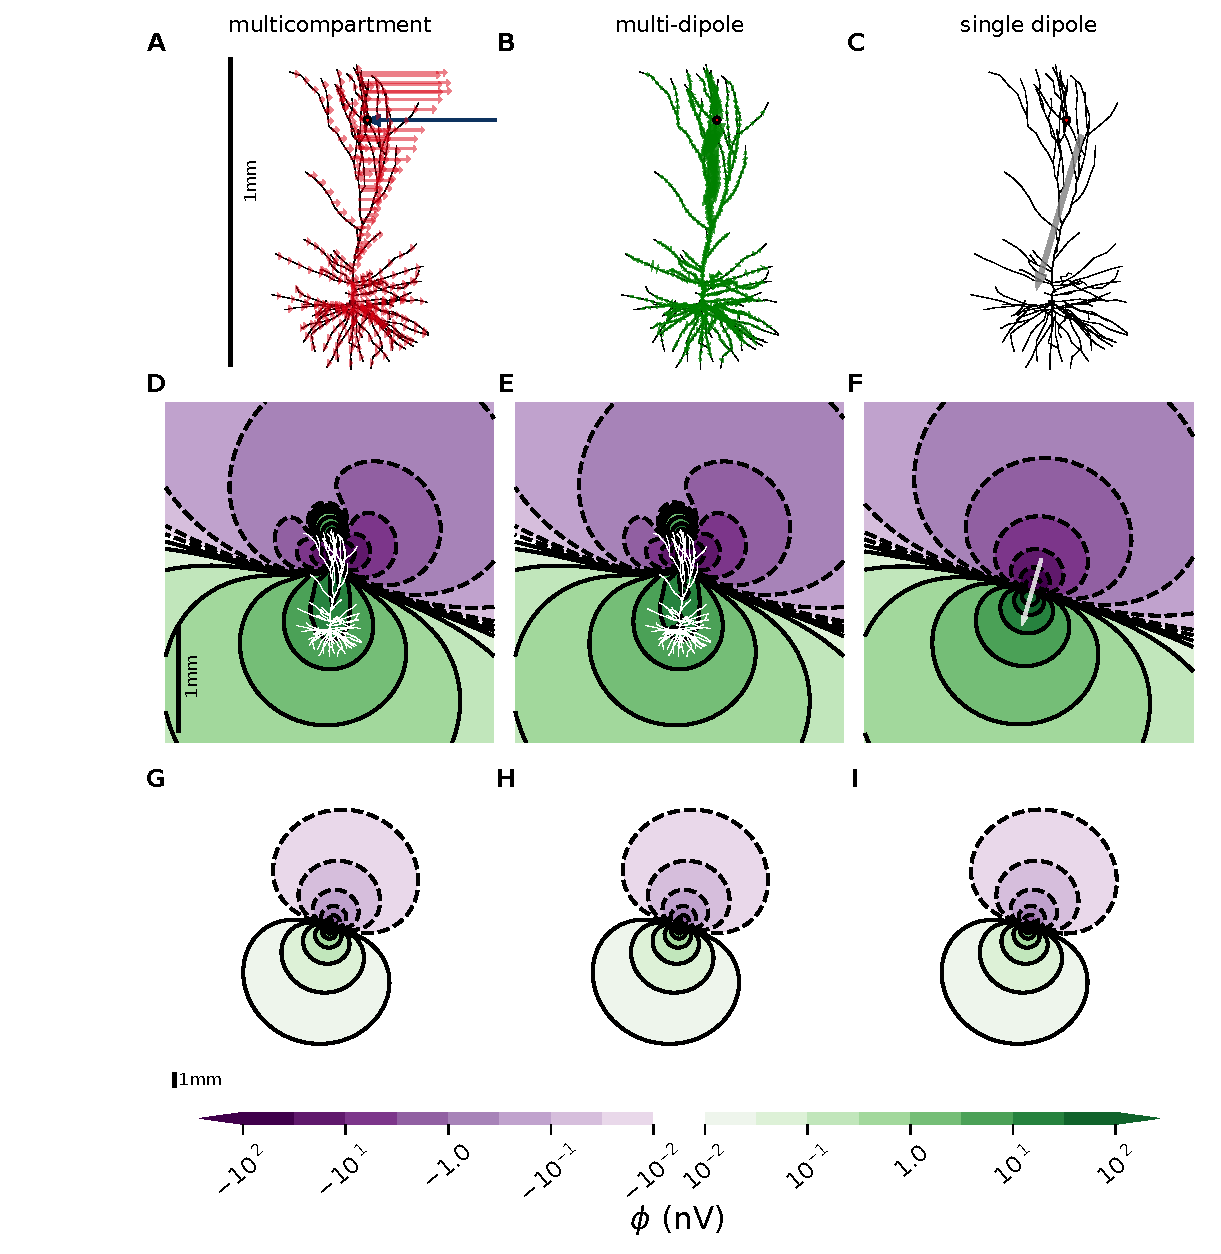
\includegraphics[width=1.0\textwidth]{fig_dipole_field}
	\caption{\textbf{Extracellular potentials becomes dipolar in the far field limit.}. 
	\textbf{A}: Layer 2/3 pyramidal cell from human \citep{EYAL2016} with an excitatory synapse placed on apical dendrite (red dot), and the resulting transmembrane currents for each compartment (blue and red arrows for negative and positive currents respectively).
	\textbf{B}: Green arrows represent the current dipole moments between neighboring neural compartments.
	\textbf{C}: Gray arrow illustrates the total current dipole moment, that is, the sum of the dipoles in B.
	\textbf{D-F}: Extracellular potential in immediate proximity of the neuron, computed with the compartment-based approach, multi-dipole approach and single-dipole approximation, respectively.
	\textbf{G-I}: Same as D-F, but at a larger spatial scale (zoomed out). See $1$~mm scalebar in panel A, D and G.
	}
	\label{fig:dipole_field}
\end{figure}


\subsection{Single-dipole approximation is justified for EEG, but not ECoG signals}\label{subsec:cb_db_comp_4s}
The ECoG and EEG signals are strongly affected by the very different conductivities of the CSF, skull and scalp \citep{NUNEZ2006}, and therefore, to test the applicability of the single-dipole approximation for computing ECoG and EEG signals, we used the four-sphere head-model \citep{NAESS2017, HAGEN2018, HAGEN2019}. 

For different positions of a single conductance-based excitatory synaptic input to the human cortical layer 2/3 pyramidal cell model \citep{EYAL2016}
(Fig.~\ref{fig:compare_multi_single_dipole}\textbf{A}), we calculated the electric potential from the top of the cell to the top of the head, using both the multi-dipole approach and the single-dipole approximation (Fig.~\ref{fig:compare_multi_single_dipole}\textbf{B}). As expected we found that synaptic input to the distal apical dendrite gave larger potentials than synaptic input to the proximal apical dendrite due to the larger current dipole moment \citep{LINDEN2010, AHLFORS2015}, and that in both cases the potential was strongly attenuated by crossing the different layers of the head model, most strongly across the low-conducting skull (Fig.~\ref{fig:compare_multi_single_dipole}\textbf{B}). 

We observed only small differences between the multi-dipole approach and the single-dipole approximation for the distal synaptic input, while for the proximal synaptic input we observed a substantial difference directly above the cell model, that was decreased along the path towards the top of the head (Fig.~\ref{fig:compare_multi_single_dipole}\textbf{B}). We quantified these differences by looking at the relative error, and found that for the distal synaptic input the relative error was 20.0(?) \% and 1.0(?) \% at the position of the ECoG and EEG electrodes respectively, while for the proximal synaptic input the relative error was 80.0(?) \% and 20.0(?) \% at the position of the ECoG and EEG electrodes respectively (Fig.~\ref{fig:compare_multi_single_dipole}\textbf{C})
\tvnnote{Solveig: Can you find exact numbers here?}. 

In other words, the single-dipole approximation results in substantial errors at the position of the ECoG electrodes in both cases, but appears well-justified at the position of the EEG electrodes for some synaptic locations. In fact, we found that the relative error of the single-dipole approximation was strongly increased for synaptic locations $\sim$ 300~$\si{\um}$ above the soma (Fig.~\ref{fig:compare_multi_single_dipole}\textbf{D}). 
This point can be considered a 'center-of-gravity' for the cells transmembrane currents  \citep{LINDEN2010, AHLFORS2015}, meaning that for a synaptic input at this location, equally much of the return current will be above and below the synaptic input, resulting in a very weak current dipole moments (Fig.~\ref{fig:compare_multi_single_dipole}\textbf{E}).
This demonstrates that the relative error of the single-dipole approximation is negatively correlated with the amplitude of the current dipole moment (Fig.~\ref{fig:compare_multi_single_dipole}\textbf{F}), indicating that for large numbers of synaptic input, the total error of the single-dipole approximation can be expected to be small.

%We tested the applicability of the single-dipole model for computing ECoG and EEG signals, using the inhomogeneous four-sphere head-model. Since the four-sphere model takes current dipole moments as input, the multi-dipole model was used as ground truth. The Hay cell with conductance-based  exponential synaptic input was modeled with $30$ different input locations. Panel \textbf{D} of Figure~\ref{fig:compare_multi_single_dipole} show that apical synaptic input gives the largest current dipole moments. Moreover, panel \textbf{E} and \textbf{F} illustrate how relative errors for single-dipole model decay as function of dipole strength for ECoG and EEG signals. From panel \textbf{B} and \textbf{C} we can see how electric potential and relative error of single-dipole model fall as a function of distance from top of neuron to measurement electrode. The relative errors of the single-dipole model are higher for ECoG than for EEG signals. \snnote{give some example here!}
\tvnnote{Did we also try current-based synapse? I think we should, so we can say it didn't matter.}
\begin{figure}[H]
	\centering
	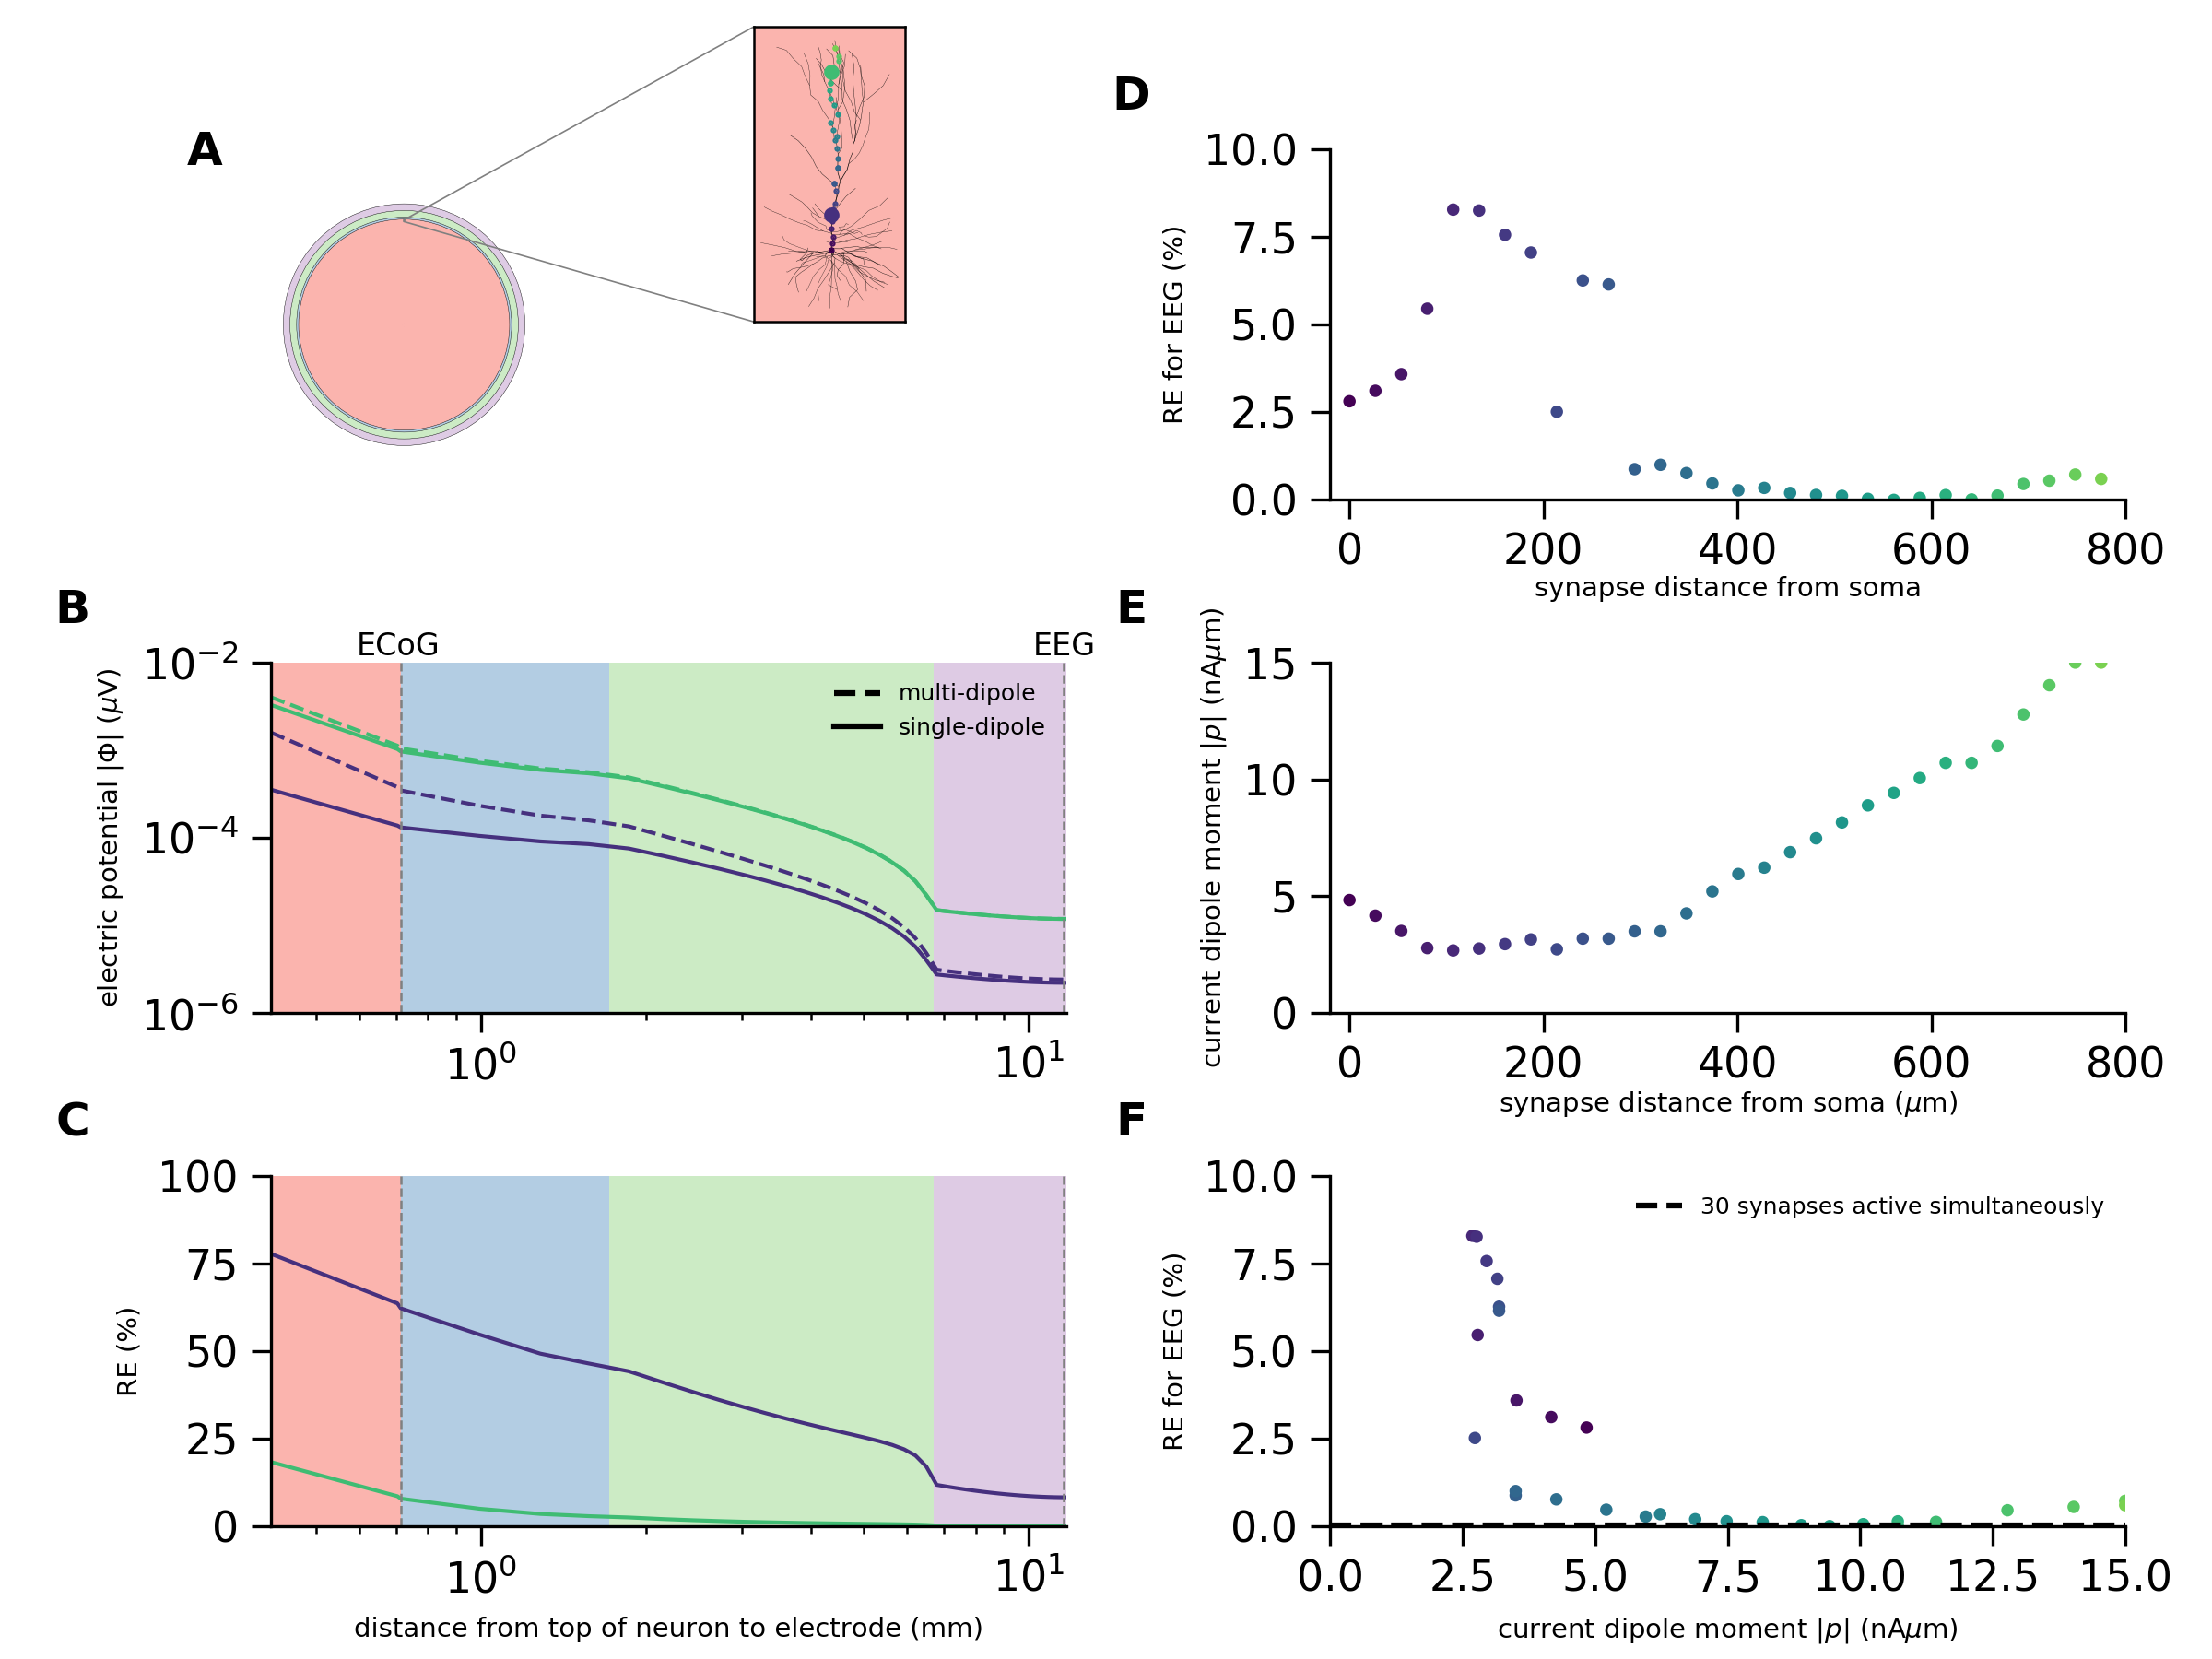
\includegraphics[width=1.0\textwidth]{fig_compare_multi_single_dipole_segev.png}
	\caption{\textbf{Single-dipole approximation is justified for EEG but not ECoG signals}. 
	\textbf{A}: Illustration of four-sphere head model, where the pink, blue, green and purple spherical shells represent the brain, CSF, skull and scalp respectively, and the inset shows the human layer 2/3 neuron \citep{EYAL2016}. $30$ simulations with a single synaptic input were performed for varying input locations, see colored dots.
	\textbf{B}: Magnitude of extracellular potential, $|\phi|$, as function of distance from the top of the neuron, shown for two simulations with synaptic input locations marked by large colored dots in inset of A. Dashed lines show extracellular potentials computed with multiple dipoles, and full lines show single-dipole calculations. \tvnnote{Is the potential at a given timestep, or is it max? Should be mentioned here I think.}
	\textbf{C}: Relative error, RE, comparing the single-dipole model to the multi-dipole model, as function of distance from top of neuron to measurement point.
	\textbf{D}: Magnitude of current dipole moment, $|\mathbf{p}|$, as function of distance from soma to synaptic input location.
	\textbf{E}: Relative error, RE, showing how single-dipole model deviates from multi-dipole model results as function of distance from soma to synapse location.
	\textbf{F}: Relative error, RE, showing how single-dipole model deviates from multi-dipole model results as function of magnitude of current dipole moment, $|\mathbf{p}|$.
	\tvnnote{Suggestion: How about running another simulation with all synapses active simulataneously, calculate the relative error, and add it to this panel (F) as a horizontal line? We would expect this to give a small error, helping to illustrate our point of the EEG being dominated by low-error dipoles.}
	}
	\label{fig:compare_multi_single_dipole}
\end{figure}

\subsection{Compact description of EEG contribution simplifies analysis}\label{subsec:compact}
%In the previous section we showed that the single-dipole approximation was applicable for calculation of EEG signals from a single synaptic input to a human cortical Layer 2/3 cell model, and we now expand this to three different cell types (Fig.~\ref{fig:eeg_compare_cell_types}\textbf{A}), each receiving a large number of synaptic inputs arriving in waves with specific target regions on the cells (Fig.~\ref{fig:eeg_compare_cell_types}\textbf{B}).
In the previous section we showed that the single-dipole approximation was applicable for calculation of EEG signals, and in this section we demonstrate that the single-dipole approximation can substantially simplify the analysis of the biophysical origin of the EEG signal.

\subsubsection{Single-dipole approximation simplifies estimate of EEG contribution}

Pyramidal cells have a preferred orientation along the depth axis of cortex (here the $z$-axis), and the direction of the current dipole moment, $\mathbf{p}$, can be expected to align with this axis since
radial symmetry will tend to make the orthogonal components ($p_x$, $p_y$) cancel \citep{HAGEN2018}. 
In contrast, interneurons show much less of a preferred orientation
(cite), and are therefore not expected to give any meaningful contribution to the EEG signal (cite) (except indirectly through input to pyramidal cells).
We illustrated this by applying the single-dipole approximation to three different cell types (Fig.~\ref{fig:eeg_compare_cell_types}\textbf{A}), each receiving a large number of synaptic inputs arriving in waves with specific target regions on the cells (Fig.~\ref{fig:eeg_compare_cell_types}\textbf{B}).

For the previously used human layer 2/3 cell from \cite{EYAL2016},
receiving a wave of 1'000 excitatory synaptic inputs that were restricted to the uppermost 250(?)~$\si{\um}$ of the cell (time=50~ms; Fig.~\ref{fig:eeg_compare_cell_types}\textbf{B}), we observed a negative deviation of $p_z$ (Fig.~\ref{fig:eeg_compare_cell_types}\textbf{C}). For basal synaptic input (time=100~ms; Fig.~\ref{fig:eeg_compare_cell_types}\textbf{B}), the polarity of $p_z$ was instead positive, but of slightly lower amplitude than for apical input, as can be expected because the large area of the somatic region will cause strong return currents in the immediate vicinity of the synaptic inputs, and therefore an overall weaker current-dipole moment.

A 1'000 synaptic inputs that were uniformly distributed across the cell membrane with area-weighted probability (time=150~ms; Fig.~\ref{fig:eeg_compare_cell_types}\textbf{B}), only gave rise to small ripples in $p_z$, due to the strong cancellation of current dipoles of opposite polarity. It is sometimes assumed that excitatory input is relatively uniformly distributed onto pyramidal cells, while inhibitory input is more directed to the perisomatic region (cite), and we found that the combination of the previously described wave of uniformly distributed synaptic input combined with perisomatic inhibitory inputs gave rise to a clear negative response in $p_z$ (time=200~ms; Fig.~\ref{fig:eeg_compare_cell_types}\textbf{B}), as would be expected from the inhibitory basal input in isolation.

For a rat cortical layer 5 pyramidal cell model \citep{HAY2011} with 10 active conductances and capability for both somatic and dendritic spikes (note that for now the synaptic input was subthreshold), the resulting current dipole moment was very similar in shape, but larger in amplitude, which was expected because the longer apical dendrite will tend to give larger current dipole moments. 

Lastly, we used a rat cortical layer 5 interneuron model (Fig.~\ref{fig:eeg_compare_cell_types}\textbf{A}; \cite{MARKRAM2015}), but since the dendrites of interneurons are not structured into the same distinctive sones as pyramidal cells, all synaptic input was uniformly distributed, and therefore caused very small net current dipole moments.

Note that in all cases, the EEG signal is nearly fully described by the single-dipole $p_z$, that is, a single time-dependent array, which corresponds to a massive simplification in understanding the biophysical origin of the EEG signal, compared to considering the transmembrane currents and position of each cellular compartment. 


%We found in the previous section that the single-dipole approximation was applicable for calculation of EEG signals, but we have not yet demonstrated its usefulness for modelling and understanding the EEG.


\tvnnote{Solveig: Could you perhaps run the simulations in Figure 3 with the multi-dipole approach as well, so we can look at the error for the different waves and cells? I'm not sure it needs to be in the figure, but it would be good to give a maximum relative error I think ('relative' with respect to the maximum signal: error / max(abs(sig))). When writing this, it feels like our verification is a bit weak still.
Maybe it would make sense to add the multi-dipole EEG as dashed lines in panel D as well?
}

\begin{figure}[H]
	\centering
	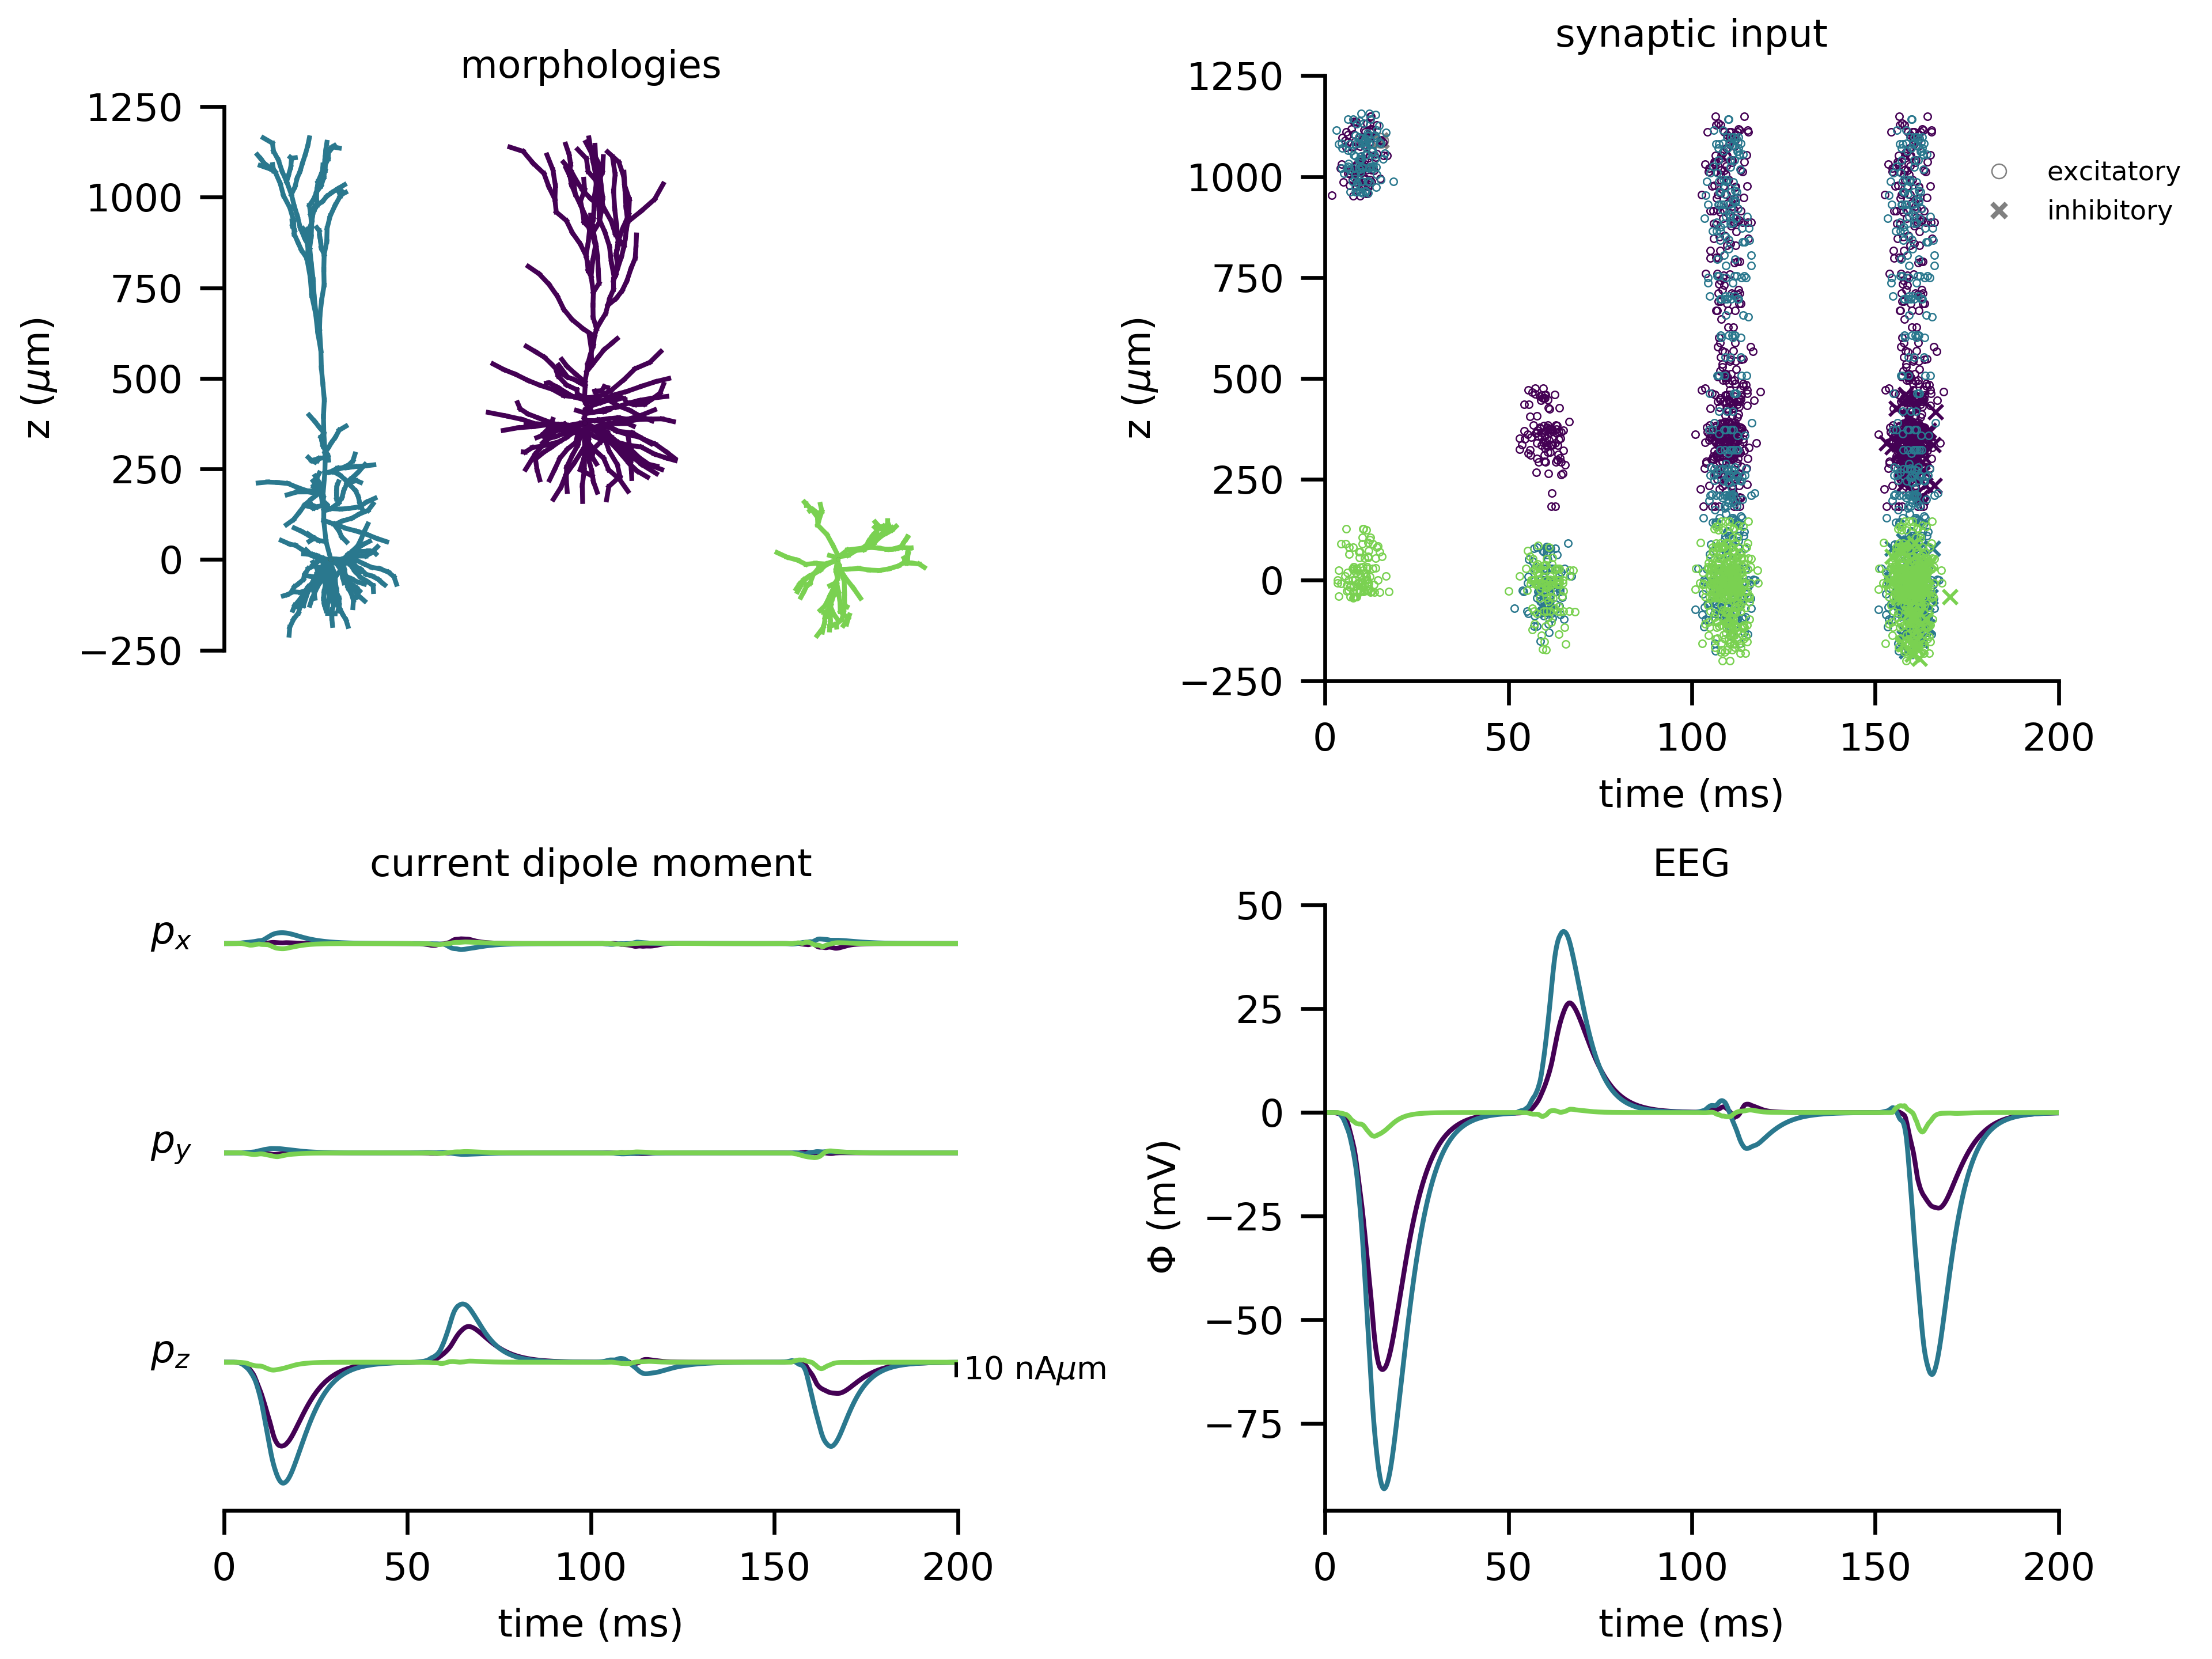
\includegraphics[width=0.8\textwidth]{fig_compare_neurons_l5ChC.png}
	\caption{\textbf{EEG signals and current dipole moment from three different cell types with various synaptic input}.
	\textbf{A}: 2D plots of the morphologies of the Hay cell (blue), the Segev cell (purple) and the \sntxt{!interneuron!} (green). All panels use the same colors for data from each cell type.
	\tvnnote{If we use the human L2/3 cell for Fig 1 and 2, I think it should come first (be the leftmost cell in panel A) here.}
	\tvnnote{Could we have names under each cell in panel A? For example ``rat L5 PC'',
	``human L2/3 PC'', and ``rat L5(?) IN''}
	\textbf{B}: Each dot represents an excitatory synaptic input at a specific time (x-axis) at a specific height of the neuron (z-axis, corresponding to panel A) for a specific cell type (color). The crosses mark inhibitory synaptic input. The four input bulks represent 1) apical excitatory input, 2) basal excitatory input, 3) homogeneously spread-out excitatory input and 4) homogeneously spread-out excitatory input and inhibitory basal input.
	\tvnnote{I suggest to add thin dotted vertical lines in the center of each wave,
	and writing ``apical input'', ``basal input'', ``uniform input'', 
	``uniform + perisomatic inhibitory input''.}
	\tvnnote{I also suggest to move the center of the waves to locations that has ticks: 50, 100, 150, 200}
	\textbf{C}: The x-, y- and z-components of the current dipole moment $\mathbf{p}$ for the three different cell types.
	\textbf{D}: EEG signals, $\phi$ from the three cell types computed with the four-sphere model.
	}
	\label{fig:eeg_compare_cell_types}
\end{figure}


\subsubsection{Current dipole moment expose dendritic calcium spikes}

\cite{SUZUKI2017} recently demonstrated that dendritic calcium spikes could be recorded at the cortical surface with amplitudes of similar magnitude as the contribution from synaptic inputs. This demonstrates that active conductances may play an important role in shaping ECoG and EEG signals, and also suggests that information might be present in such signals which can be used in new ways to study the learning mechanisms associated with dendritic calcium spikes (cite). We found that the single-dipole approximation provides a convenient way of investigating the EEG-contribution of such dendritic calcium spikes.

The previously introduced rat layer 5 cortical pyramidal cell model from \cite{HAY2011} can exhibit dendritic calcium spikes.
When this cell model received a single excitatory synaptic input to the soma (Fig.~\ref{fig:ca_spike}\textbf{A}, blue dot) strong enough to elicit a somatic action potential (Fig.~\ref{fig:ca_spike}\textbf{B1}, blue), a small depolarization was also visible in the apical dendrite but no dendritic calcium spike was initiated (Fig.~\ref{fig:ca_spike}\textbf{B1}, orange). If instead the same somatic synaptic input was combined with an additional excitatory synaptic input to the apical dendrite 400~$\si{\um}$ away from the soma (Fig.~\ref{fig:ca_spike}\textbf{A}, orange dot), a dendritic calcium spike was initiated, which also induced two additional somatic spikes (Fig.~\ref{fig:ca_spike}\textbf{C1}).

The simulated extracellular potential 30~$\si{\um}$ away from the soma had the shape of stereotypical extracellular action potentials in both cases, that is, a sharp negative peak followed by a broader and weaker positive peak (Fig.~\ref{fig:ca_spike}\textbf{B2, C2}), and the slow dendritic calcium spike was not reflected in the extracellular potential close to the soma (Fig.~\ref{fig:ca_spike}\textbf{C2}).
We found that for the case with only a somatic spike and no calcium spike, the single-cell current dipole moment resembled the inverse of the extracellular potential (Fig.~\ref{fig:ca_spike}\textbf{B3}), while for the case with both somatic and dendritic spiking, a pronounced slow component was also present in the single-cell current dipole moment (Fig.~\ref{fig:ca_spike}\textbf{C3}).
Note that somatic action potentials are typically not expected to contribute significantly to EEG signals (cite, but see \cite{TELENCZUK2015}), because the very short duration of spikes with both a positive and a negative phase implies that extreme synchrony is needed for spikes to sum constructively. Indeed, we found that when we calculated the sum of 1'000 instanced of the single-cell current dipole moment that was jittered (shifted) in time (normally distributed, standard deviation=10~ms), the case with the dendritic calcium spike has a $6.6$-fold larger maximum amplitude than the case with
only the somatic spike (Fig.~\ref{fig:ca_spike} \textbf{B4} versus \textbf{C4}, 
$\mathrm{max}|\mathbf{p}$| = 30.8~$\si{\uA}\cdot\si{\um}$ and 204.2~$\si{\uA}\cdot\si{\um}$ respectively). This demonstrates that dendritic calcium spikes are much more capable of summing constructively for a population of cells, and substantiates the role of dendritic calcium spikes in affecting ECoG/EEG/MEG recordings. 
\tvnnote{Although our Ca-spikes appear quite different in shape to the ones demonstrated by Suzuki and Larkum (2017), who (in defence of our results) reported an 'unexpected shape'}

It might initially seem surprising that the dendritic calcium spike is so strongly reflected in the single-cell current dipole moment, given that the transmembrane currents associated with the somatic action potential are much larger than those associated with the dendritic calcium spike: the maximum amplitude of the transmembrane currents of the somatic compartment was 45.1~$\si{\nA}$, compared to just 0.30~$\si{\nA}$ for the compartment with the apical synaptic input (Fig.~\ref{fig:ca_spike}A, blue and orange dots). However, the current dipole moment is given as the product between the amplitude of the current and the separation between the source and sink ($\mathbf{p}=I\mathbf{d}$; eq. \ref{eq:dip_trans_to_axial}), and while the currents associated with the somatic action potential will for the most part be contained within the somatic region, giving very small sink/source separations, the currents associated with the dendritic calcium spike will be distributed over a much larger part of the cell membrane (cite?).

\begin{figure}[H]
	\centering
	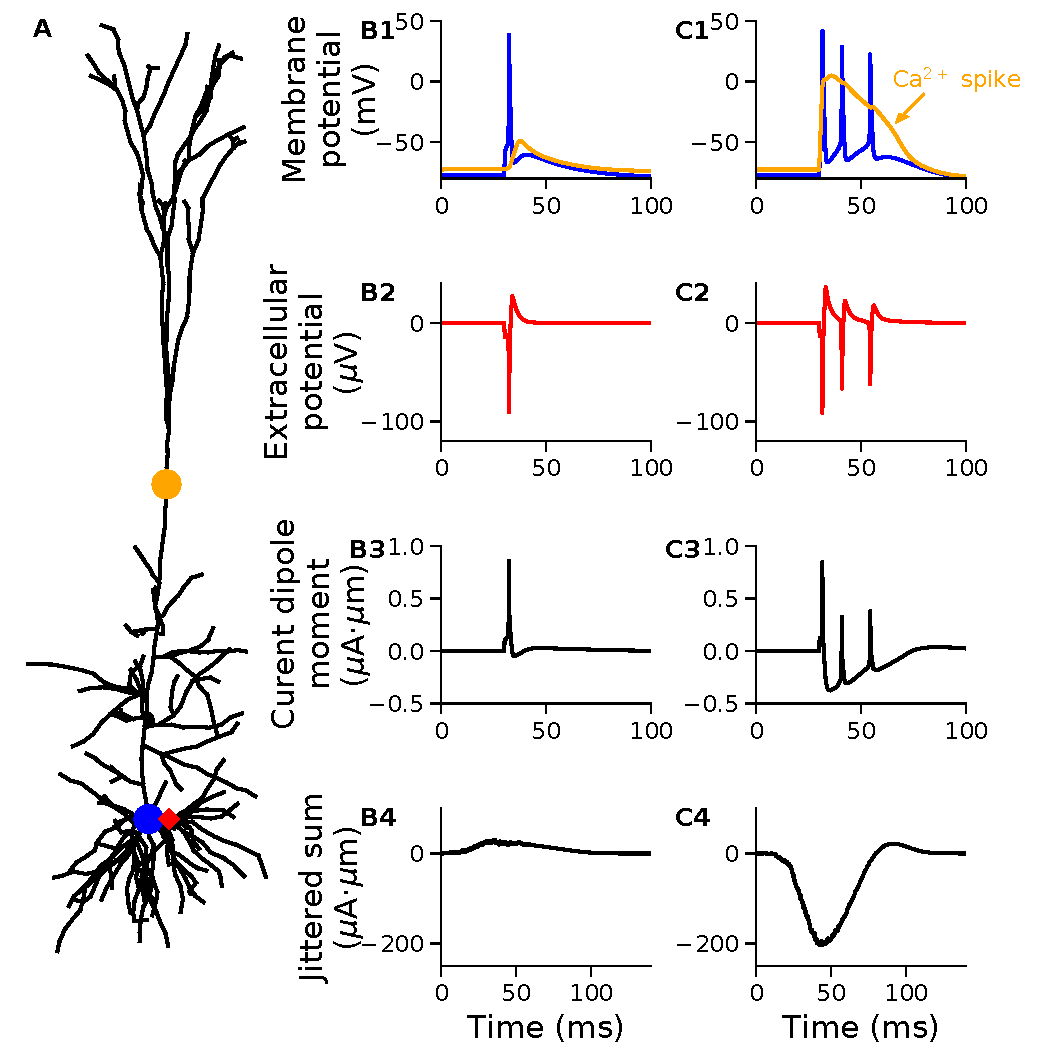
\includegraphics[width=0.6\textwidth]{ca_spike_hay}
	\caption{\textbf{Current dipole moment expose dendritic calcium spikes.}
	\textbf{A}: Layer 5 cortical pyramidal cell model from rat \citep{HAY2011}, receiving either a single excitatory synaptic input to the soma evoking a single somatic action potential (blue dot, results in \textbf{B1-4}), or in addition an excitatory synaptic input to the apical dendrite, evoking a dendritic calcium spike and two additional somatic spikes (orange dot, results in \textbf{C1-4}). 
	\textbf{B1, C1}: Membrane potential at the two positions indicated in \textbf{A}.
	\textbf{B2, C2}: Extracellular potential 30~$\si{\um}$ away from the soma (red diamond in \textbf{A}), assuming for illustration an infinite homogeneous extracellular medium. 
	\textbf{B3, C3}: Single-cell current dipole moment. 
	\textbf{B4, C4}: Sum of 1'000 instances of the single-cell current dipole moment (from \textbf{B3, C3}), that has been randomly shifted in time with a normally distributed shift with a standard deviation of 10~ms.
	}
	\label{fig:ca_spike}
\end{figure}

\subsection{Dipole approximation for populations of cells}
We have so far only considered the EEG contributions from single cells, but real EEG signals are expected to reflect the activity of hundreds of thousands to millions of cells \citep{NUNEZ2006, COHEN2017}. 
We therefore used the large-scale point-neuron cortical microcircuit model from \cite{POTJANS2014}, in combination with the hybrid scheme for calculating LFPs and EEGs \citep{HAGEN2016}. Breifly, this model has $\sim$80'000 neurons divided into 8 different cortical populations, one excitatory and one inhibitory across four layers (L2/3 - L6), and it can exhibit different network states, including different kinds of oscillations or behaviour similar to an asynchroneous irregular network state \citep{HAGEN2016, BRUNEL2000}.
The network activity is simulated for point neurons (Fig.~\ref{fig:population}) using NEST \citep{NEST}, and synaptic input to the neurons is saved and used as synaptic input to corresponding biophysically detailed multicompartment neurons, from which the single-cell current dipole moment of each cell is obtained, together with the 


\begin{figure}[H]
	\centering
	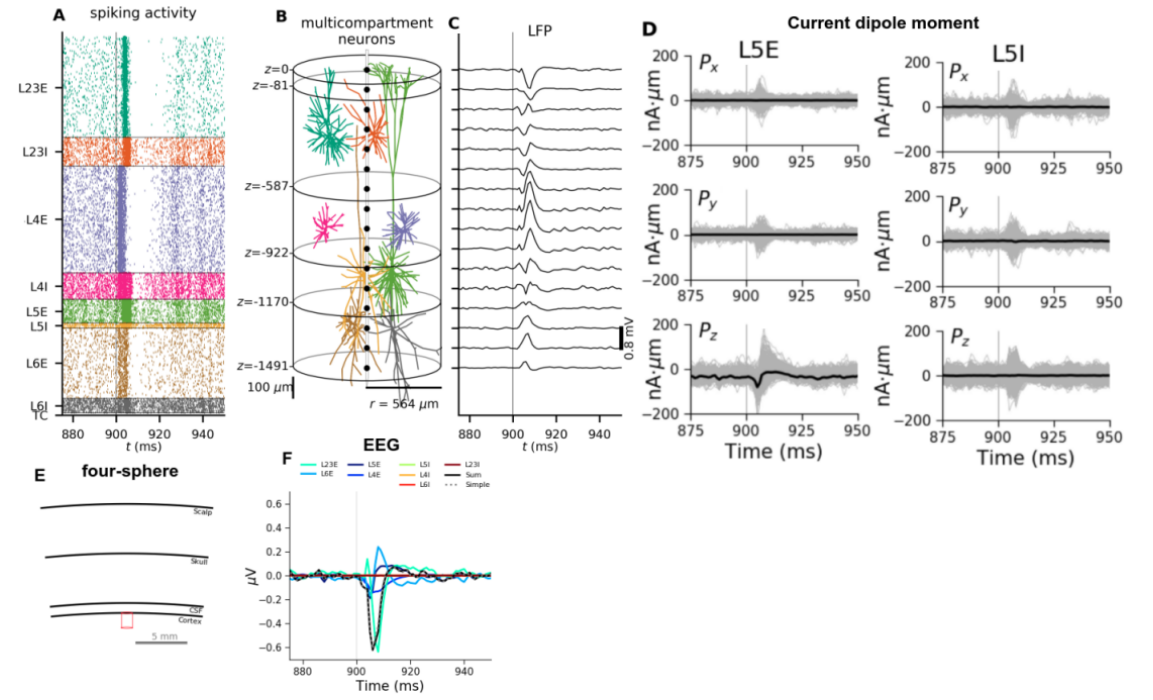
\includegraphics[width=1.0\textwidth]{hybrid_eeg}
	\caption{\textbf{Extracellular potentials becomes dipolar in the far field limit.}. 
	\textbf{A}:
	}
	\label{fig:population}
\end{figure}

\sntxt{
\begin{itemize}
	\item Because of linearity, the EEG from a neural population is the sum of all the single-cell EEG contributions. However, if the spatial extent of the neural population (~ 1 mm) is small relative to the distance to the EEG electrodes (~ 1 cm), then individual current-dipoles can be summed, e.g., for each neural sub-population, or for the entire neural population, and the EEG signal can be computed based on the summed current dipoles. This could be a very promising approach for decomposing and understanding the EEG in large-scale neural  simulations like the cortical column simulations of the HBP, the Potians-Diesman  simulations of Hagen, or the Allen brain initiative.
	\item Which populations are important? We found that the EEG calculated as the sum of the single-cell EEG contributions from the current dipoles of all ~80,000 cells, spatially distributed within a cylinder (panel B and E) was indistinguishable from the EEG calculated as the sum of the EEG from 4 population current dipoles in the center of the population. Each of these 4 current dipoles was the sum of the z-components of the current dipoles of the pyramidal cells in the different layers (panel F, L23E, L4E, L5E, L6E). We found that all pyramidal cell populations had a substantial EEG contribution, however, the largest was the L2/3 population. It should however be noted that this is not a very realistic scenario, because of current-based synapses etc.
	
\end{itemize}
	
	}
\subsection{Dipole approximation in more complex head models}
\sntxt{
\begin{itemize}
	\item Insert population dipole vector into NY head model
\end{itemize}
	}
%%%%%%%%%%%%%%%%%%%%%%%%%%%%%%%%%%%%%%%%%%%%%%%%%%%%%%%%%%%%%%%%%%%%%%%%
%%%%%%%%%%%%%%%%%%%%%%%%%%%%%DISCUSSION%%%%%%%%%%%%%%%%%%%%%%%%%%%%%%%%%
%%%%%%%%%%%%%%%%%%%%%%%%%%%%%%%%%%%%%%%%%%%%%%%%%%%%%%%%%%%%%%%%%%%%%%%%
\section{Discussion}\label{sec:discussion}


We have found that the single-cell current dipole moment is applicable for calculating a neuron's EEG-contribution, and that this approach can be helpful in estimating the relative EEG-contribution of different cell types and different modes of synaptic input, in addition to investigating 

In this formalism it is easy to investigate the contribution to the EEG signal from, e.g., different cell types, from somatic spikes, or from dendritic spikes, by only comparing the z-component of the resulting current dipoles, without the need for the added complexity of head models etc.

\begin{itemize}
\item Good paper for discussion/intro:  \cite{COHEN2017} (``too little is done to understand the origin of the EEG'')
\item Discuss value of results to ongoing large-scale simulation projects.
\item ``EEG is hard to enterpret because of large number of neuron contributing''. True, but still basically (probably) just four main sources: apical excitation/inhibition and basal excitation/inhibition to pyramidal cells, and connectivity is to a large degree fixed, meaning that we could probalby map population firing rate to EEG.
 \item Discuss relevance to \cite{MAKI2019}?
\item Discuss value of decoupling current dipole moments and head model
\item Discuss kernel from population firing rates to current dipole moment?
 \item Discuss potential impact of I$_{\rm h}$ on human EEG \citep{NESS2016, NESS2018, KALMBACH2018}.
 \item Compare to other projects like HNN (Human Neocortical Neurosolver) (\url{https://hnn.brown.edu/})
 \item Important work on the path towards a real understanding of the biophysical origin of EEGs \cite{BRUYNS2017}
\end{itemize}


% \appendix
% \section{Point-Source vs. Line-Source Dipole Moment} \label{sec:point_line_cdm}
% \tvnnote{I don't think we need to go into this.}
% Considering the single-dipole neuron model, the line-source approximation gives a more accurate estimate than the point-source approximation. This section goes into the question of whether the choice of point-source or line-source approximation has an effect on the calculation of current dipole moments.
% 
% Transmembrane currents can be expressed as the spatial integral over the linear current density $i$. Following, the current dipole moment equation from transmembrane currents \eqref{eq:ptrans} is split into x-, y- and z- components, so that $\mathbf{p}(t) = p_x(t)\mathbf{\hat{x}} + p_y(t)\mathbf{\hat{y}} + p_z(t)\mathbf{\hat{z}}$, and each direction component is written as a function of $i$:
% 
% \begin{align}\label{eq:pxpypz}
% p_x(t) &= \sum_{n=1}^N\int x_n i_n(x,t) dx, \nonumber\\
% p_y(t) &= \sum_{n=1}^N\int y_n i_n(y,t) dy, \\
% p_z(t) &= \sum_{n=1}^N\int z_n i_n(z,t) dz, \nonumber
% \end{align}
% where $N$ is the total number of compartments.
% 
% Next, an example for applying the point-source approximation to calculate the current dipole moment from a dendritic stick is outlined. We assume a straight multicompartmental dendrite model with $N$ compartments, each of length $\Delta L$, elongated in the z-direction only. Its linear current density for the point-source approximation can be expressed as follows
% 
% \begin{equation}
% i_n(z,t) = I_n(t) \delta(z - z_n),
% \end{equation}
% where $I_n(t)$ is the space-independent current component and $z_n$ is the middle position of compartment $n$, i.e., where current can leave or enter. Plugging this into Equation \eqref{eq:pxpypz}, and integrating over the length of each compartment, $\Delta L$, the following expression for $p_z$ appears:
% 
% \begin{equation}
% p_z = \sum_{n=1}^N \int_{z_n - \frac{\Delta{L}}{2}}^{z_n + \frac{\Delta L}{2}} z_n I_n(t) \delta(z - z_n)dz = \sum_{n=1}^N z_n I_n(t).
% \end{equation}
% 
% When calculating the current dipole moment using the line-source approximation, the linear current density takes the following form:
% \begin{equation}
% i_n(z,t) = \frac{I_n(t)}{\Delta L}.
% \end{equation}
% Inserting this into Equation \eqref{eq:pxpypz} gives
% 
% \begin{align}
% p_z
% & = \sum_{n=1}^N \int_{z_n - \frac{\Delta L}{2}}^{z_n + \frac{\Delta L}{2}} z \frac{I_n(t)}{\Delta L}dz \nonumber \\
% & = \sum_{n=1}^N \frac{I_n(t)}{\Delta L} \big[\frac{1}{2} z^2\big]_{z_n - \frac{\Delta L}{2}}^{z_n + \frac{\Delta L}{2}} \\
% & = \sum_{n=1}^N z_n I_n(t). \nonumber
% \end{align}
% 
% Hence, we have found that the point-source and the line-source approximations will give the exact same results when calculating current dipole moments. The simpler point-source approximation is therefore preferable.
\section*{References}
\bibliography{eeg_main}
\end{document}
